% Dynamic Programming
%
% A cartoon-like introduction to dynamic programming in sequence alignment.
% The aim is to illustrate the method, with some easy to parse examples, 
% emphasising that the method is general and mathematical, and that any 
% biology resides only in (i) the scoring scheme (substitution matrix) and (ii)
% the scientists' heads when interpreting the biology

\subsection{Dynamic Programming}
  \begin{frame}
  \frametitle{Our Goal}
  \begin{itemize}
    \item<1-> We aim to align the words
    \begin{itemize}
      \item<1-> \texttt{COELACANTH}
      \item<1-> \texttt{PELICAN}
    \end{itemize}
    \item<2-> Each identical letter (match) scores +1
    \item<2-> Each different letter (mismatch) scores -1
    \item<2-> Each gap scores -1
    \item<3-> \emph{All sequence alignment is maximisation of an alignment score} - a mathematical operation.
  \end{itemize}
\end{frame}   
   
\begin{frame}
  \frametitle{Initialise the matrix}
  \begin{center}
    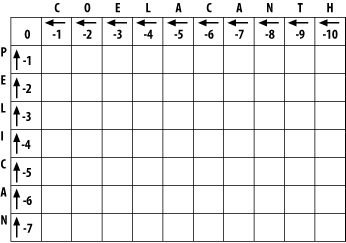
\includegraphics[width=0.65\textwidth]{images/initialise}
    \end{center}
\end{frame}   
   
\begin{frame}
  \frametitle{Fill the cells}
  \begin{center}
    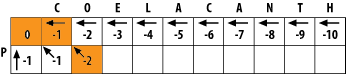
\includegraphics[width=0.65\textwidth]{images/fill_start} \\
    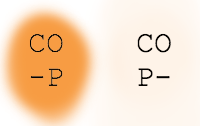
\includegraphics[width=0.3\textwidth]{images/fill_start_letters}
  \end{center}
\end{frame}     

\begin{frame}
  \frametitle{Fill the matrix -- represents all possible alignments \& scores}
  \begin{center}
    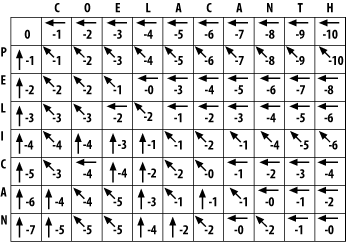
\includegraphics[width=0.65\textwidth]{images/full_matrix}
  \end{center}
\end{frame}  
   
\begin{frame}
  \frametitle{Traceback}
  \begin{center}
    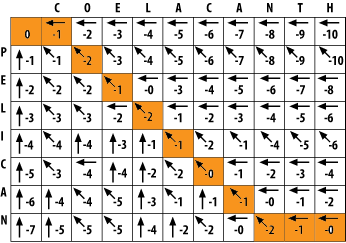
\includegraphics[width=0.65\textwidth]{images/traceback} \\
    
\includegraphics[width=0.3\textwidth]{images/traceback_sequence}         
  \end{center}
\end{frame}     

\begin{frame}
  \frametitle{Algorithms}
  \begin{itemize}
    \item<1-> Global: Needleman-Wunsch (as in example)
    \item<1-> Local: Smith-Waterman (differs from example)
    \item<2-> Biological information encapsulated \emph{only} in the scoring scheme (matches, mismatches, gaps)
    \item<3-> NW/SW are \emph{guaranteed} to find the optimal match \emph{with respect to the scoring system being used}
    \item<3-> BUT the optimal alignment is a biological approximation: no scoring scheme encapsulates biological ``truth''
    \item<3-> Any pair of sequences can be aligned: finding meaning is up to you
  \end{itemize}
\end{frame}   